\chapter{Background and Philosophy}
\label{chap:philosophy}

In physics, the speed of light, denoted $c$, is the ultimate speed
limit of the universe.  Likewise in programming, ``as fast as C'' is
often used as an indication that some programming language is as fast
as it can possibly be.  In theory it makes no sense to say that a
given programming language is ``slow'' or ``fast'', as these are
merely properties of a particular implementation of the programming
language running on a specific computer.  But in practise, it is clear
that the design of a programming language has an overwhelming
influence on the ease with which a performant implementation can be
constructed.

For decades, the design of languages such as C has permitted the
implementation of compilers that generate efficient code.  One
important reason is that the abstract machine model underlying C, a
sequential random-access register machine, can be mapped easily to
mainstream computers with little overhead.  This means that a
programmer can write code in C and have a reasonable idea of the
performance of the resulting code.  It also means that even a naive
non-optimising C compiler can generate code with good performance,
although it may require somewhat more care from the C programmer.
Indeed, C has often been described as ``portable assembly
code''.\footnote{I will using C as the main point of reference in the
  following sections, but the problems I point out are common to any
  sequential language.}

In contrast, languages whose abstract model is more different from
physical machines, so-called ``high-level languages'', cannot be as
easily mapped to real machines.  Compilers must invest considerable
effort in mapping e.g. the call-by-need lambda calculus of Haskell to
the sequential register machine~\cite{jones1992implementing}.  Even
after decades of work, high-level languages struggle to catch up to
the performance of C on the sequential random-accesss register
machine.

Of course, a cursory study of modern hardware designs show that the
sequential random-access register machine is an illusion.  The abstract
model of C may match a 70s minicomputer reasonably well, but it is
increasingly diverging from how modern computers are constructed.
This is not despite lack of effort on behalf of the hardware
designers: due to the massive popularity (and therefore economic
significance) of C-like languages, manufacturers have attempted to
prolong the illusion of the sequential random-access machine for as long as
possible.

Unfortunately, while C may be exceeded (as I hope to show in this
thesis), $c$ is a harder nut to crack.  The machine on which I am
typing contains a CPU with a clock frequency of $2.3GHz$,
corresponding to a clock cycle taking $0.43ns$.  Given that $c$ is
approximately $3\cdot10^{8}m/s$, light moves approximately $13cm$ in
the the time the CPU takes to perform a clock cycle, thus physically
limiting the distance a single piece of information can travel in a
single cycle.

Another physical limitation is power dissipation: roughly, the power
usage of the transistors in a processor is roughly proportional to the
square of its clock frequency\fixme{cite}.  This prevents an increase in clock
frequency unless we can compensate with an increase in the efficiency
of the transistors.  For a sequential machine that executes
instructions in exactly the order they are given, the only way to
speed up execution of a program is to increase the rate at which
instructions are executed.  If we can double the rate at which
instructions are processed, we in effect halve the time it takes to
execute some program (assuming no memory bottlenecks, which I will
discuss later).

In the popular vernacular, \textit{Moore's Law} is typically rendered
as ``computers double in speed every two years''.  But actually, the
law states that \textit{transistor density} doubles every two years
(implying that transistors become smaller).  Moore's Law does not
state that the enlargened transistor budget translates
straightforwardly to improved performance, although that was indeed
the case for several decades.  This is due to another law,
\textit{Dennard scaling}, which roughly states that as transistors get
smaller, their power density stays constant.  Taken together, Moore's
Law and Dennard scaling rougly say that we can put ever more
transistors into the same physical size, and with the same power usage
(and thus heat generation).

The reduction in power usage per transistor granted by Dennard scaling
permitted a straightforward increase in CPU clock frequency.  Roughly,
every time we cut the power consumption of a transistor in half via
shrinkage, we can increase the clock frequency by 50\%.  For a
sequential computer, this translates into a 50\% performance increase.
We can partially circumvent the limits of $c$ by using techniques such
as \textit{pipelining}.  While it is clear that Moore's Law will
eventually stop, or else transistors would eventually be smaller than
a single atom, this is not the issue that has hindered the illusion of the
sequential machine.

The problem is that Dennard scaling began to break down around 2006.
Physical properties of the circuit material leads to increased current
leakage at small sizes, causing the chip to heat up.  Simply pushing
up the clock frequency is no longer viable.  Instead, chip
manufacturers use the transistor budget on increasing the amount of
work that can be done in a clock cycle through various means:

\begin{description}
\item[Increasing the size of caches.] One significant problem with
  modern computer designs is that processors are significantly faster
  than the memory from which they get their data.  As a rule of thumb,
  accessing main memory incurs a latency of $100ns$ - likely hundreds
  of clock cycles on a current CPU.  This so-called \textit{memory
    wall} can be circumvented by the addition of caches that store
  small subsets of the larger memory.  Heuristics, usually based on
  temporal locality, are useed to determine which parts of the larger
  memory are stored in the caches.  High-performance CPUs can use
  several layers caches, each layer being larger and slower than the
  former.
\item[Inferring instruction-level parallelism.]  While the semantics
  of a sequential CPU is that instructions are executed one after
  another, it is often the case that two instructions to not have
  dependencies on one another, and thus can be executed in parallel.
  CPUs even perform \textit{out-of-order} execution where later
  instructions are executed before earlier ones, if the latter
  instruction has no dependence on the latter.
\item[Explicit parallelism at the hardware level.]  The two former
  techniques try to masquerade the fact that the sequential machine
  model is increasingly physically untenable.  Another approach is to
  explicitly provide programmers with hardware support for parallel
  execution.  This most famously takes the form of adding additional
  CPU cores, each of which processes a sequential stream of
  instructions, but an equally important technique is to add
  \textit{vector instructions} that operate on entire vectors of data,
  rather than single values.  As an example, the newest Intel AVX-512
  vector instruction set provides instructions that operate on entire
  512-bit vectors (for example, 16 single precision floating point
  values).  Such instructions dramatically increase the amount of work
  that is done in a single clock cycle.
\end{description}

These techniques are all based on merely extending and improving the
classic CPU design.  While code may have to be re-written to take
advantage of certain new hardware features (such as multiple cores or
vector instructions), the programming experience is not too dissimilar
from programming sequential machines.  This is not necessarily a bad
thing: sequential machines are easy to reason about, generous in their
support of complex control flow, and have a significant existing base
of programmer experience.

However, the notion that C is ``portable assembly'' begins to crack
noticeably even at this point.  C itself has no built-in notion of
multi-threaded programming, nor of vector operations, and thus vendors
have to provide new programming APIs (or language extensions) for
programmers to take advantage of the new (performance-critical)
machine features.  Alternatively, C compilers must perform significant
static analysis of the sequential C code to find opportunities for
vectorisation or multithreading.  In essence, the compiler must
reverse engineer the sequential statements written by the programmer
to reconstruct whatever parallelism may be present in the original
algorithm.

The problem is that C was carefully designed for a particularly class
of machines; a machine no longer resembled by modern high-performance
computers.  Thus, the \textit{impedance mismatch} between C and
hardware continues to grow, with little sign of stopping.  This
mismatch becomes acute when we move away from the comparatively benign
world of multicore CPUs and into the realm of massively parallel
processors.

\section{Massively Parallel Machines}

To a large extent, mainstream CPUs favour programming convenience,
familiarity, and backwards compatibility over raw performance.  We
must look elsewhere for examples of the kind of hardware that could be
built if we were willing to sacrifice traditional sequential notions
of sequential programming.

For as long as there has been computers, there have been parallel
computers.  Indeed, if we think back to the very earliest computers,
the human ones made of flesh and blood, parallelism was the
\textit{only} way to speed up a computation.  You were unlikely to
make a single human computer much faster through training, but you
could always pack more of them into a room.  However, with the rise of
electrical computers, and in particular the speed with which
sequential performance improved, parallelism dwindled into the
background.  Certainly, you could have two computers cooperate on
solving some problem, but the programming difficulties involved made
it more palatable to simply wait for a faster computer to enter the
market.  Only the largest computational problems were worth the pain
of parallel programming.\footnote{\textit{Concurrency} was alive and
  well, however, due to its significant importance in operating
  systems and multiprocessing.  But most concurrent programs were
  executed on sequential machines, with the illusion of concurrency
  formed through multiplexing.  Many of the techniques developed for
  concurrent programming are also applicable to parallel programming,
  although concurrency tends to implicitly focus on correctness over
  performance on some specific machine.}

Several interesting parallel computers were designed for
\textit{high-performance computing} (HPC) applications.  One of the
earliest and most influential was the Cray-1 from 1976, which was the
first vector processor\fixme{cite}.  Only about 100 were sold, but this is a large
number for a high-end supercomputer.  A different design was the CM-1
from 1985, which was based on a computer containing a large number of
simple 1-bit microprocessors.  The CM-1 proved difficult to program
and was not a success in the market, but was the first example of a
\textit{massively parallel machine}\fixme{cite}.

In the 90s, consumer demand for increasing visual fidelity in video
games led to the rise of the \textit{graphics processing unit} (GPU),
for accelerating graphical operations that would be too slow if
executed on the CPU.  Initially, GPUs were special-purpose
non-programmable processors that could only perform fixed graphical
operations.  Over time, the need for more flexibility in graphical
effects lead to the development of programmable \textit{pixel
  shaders}, first seen in the NVIDIA GeForce 3 in 2000.  Roughly,
pixel shaders allowed an effect to be applied to every pixel of an
image - for example, looking at every pixel and add a reflection
effect to those that represent water.  Graphical operations such as
these tend to be inherently parallel, and as a result, GPU hardware
evolved to support efficient execution of programs with very simple
control flow, but a massive amount of fine-grained parallelism.
Eventually, GPU manufacturers started providing APIs that allowed
programmers to exploit the parallel computational power of the
now-mainstream GPUs even for non-graphics workloads, so-called
\textit{general-purpose GPU programming} (GPGPU).  The most popular
such APIs are CUDA~\cite{cuda} from NVIDIA, and
OpenCL~\cite{Stone:2010:OPP:622179.1803953}.

GPUs are not the only massively parallel machines in use.  However,
their great success, their availability, the difficulty in programming
them, and their potential compute power makes them excellent objects
of study for researchers of parallel programming models.  In this
work, I focus on the details of GPUs over other parallel machines.
However, a central thesis of the work is that modern hardware is too
complicated and too diverse for low-level programming by hand to be
viable.  I will introduce a high-level hardware-agnostic programming
model, and describe its efficient mapping to GPUs.  The implication is
that if the model can be mapped efficiently to a platform as
restricted as GPUs, it can probably also be mapped to other parallel
platforms, such as multicore CPUs, clusters, or maybe even FPGAs.

\subsection{Basic Properties of GPUs}

The performance characterictics and programming model of modern GPUs
is covered in greater detail on~\ref{chap:hardware}, but a basic
introduction is given here, in order to give an idea of the
difficulties involved in retrofitting sequential languages for GPU
execution.

GPUs derive their performance from an execution model called
\textit{single instruction multiple thread} (SIMT), which is very
similar to the \textit{single instruction multiple data} model.
Roughly, threads are not fully independent, but grouped into bundles
that all execute the same operations on different parts of a large
data set.  For example, on an NVIDIA GPU, threads are bundled into
\textit{warps}, of 32 threads each, that execute in lockstep, and
which form the unit of scheduling.  This execution is highly suited
for dense and regular computations, such as the ones found in linear
algebra, but less so for irregular and branch-heavy computations such
as graph algorithms.

A GPU is still subject to the laws of physics, and there is therefore
a significant latency between issuing a memory read, and actually
receiving the requested data (the memory wall).  On a CPU, a hierarchy
of caches is used to decrease the latency, but a GPU uses aggressive
\textit{simultaneous multithreading}, where a thread that is waiting
for a memory operation to complete is de-scheduled and another thread
run in its place.  This scheduling is done entirely in hardware, and
thus does not carry the usual overhead of context switches.  This
scheduling is not done on each thread in isolation, but on entire
32-thread warps.  Thus, while a GPU may be only have enough
computational units (such as ALUs) to execute a few thousand parallel
instructions per clock cycle, tens of thousands of threads may be
necessary to avoid the computational units being idle while waiting
for memory operations to finish.  As a result of this design, memory
can also be optimised for very high bandwidth at the expense of
latency, and it is not unusual for GPU memory buses to support
bandwidth in excess of $300GiB/s$ (although as we shall discuss in
Chapter~\ref{chap:hardware}, specific access patterns must be followed
to reach this performance).

GPUs have many limitations that hinder traditional programming
techniques and languages:

\begin{itemize}
\item GPUs function as \textit{co-processors}, where code is
  explicitly uploaded and invoked.  A GPU program is typically called
  a \textit{GPU kernel}, or just \textit{kernel}.
\item The amount of threads necessary implies that each thread can use
  only relatively few registers and little memory (including stack
  space).
\item The lockstep execution of warps, as well as the very small
  per-thread stack size, prevents function pointers and recursion.
\item GPUs cannot directly access CPU memory, and so data must
  manually be copied to and from the GPU.\footnote{This is changing
    with the newer generation of GPUs.}
\item The memory hierarchy is explicit.  While a small amount of cache
  memory is often present, obtaining peak performance depends on
  judicious use of programmer-managed on-chip memory.
\item Memory allocation is typically not possible while executing a
  GPU program.  All necessary memory must be pre-computed before
  starting GPU execution.
\item Generally no support for interrupts or signals.
\end{itemize}

The mismatch between the abstract machine model of C and GPU
architectures is clear.  While current GPU programming APIs do in fact
use a restricted subset of C (or C++ in the case of CUDA) for
expressing the per-thread code, it is the programmmer's responsibility
to orchestrate their execution.  This involves organising
communication between the tens of thousands of threads that are needed
to saturate the hardware, with both correctness and performance easily
suffering under even small mistakes---a tall order, and the compiler
offers little help.  In practise, this renders GPU programming the
domain of experts, and off-limits to most programmers, except through
the use of restricted libraries offering pre-defined primitives.

\section{A Parallel Programming Language}

We need a better programming model; one that does not have as
fundamental a mismatch between its execution model and parallel
hardware.  This does not mean we need a low-level language, or a
specialised GPU language.  Rather, we should \textit{increase} the
level of abstraction, and stop overspecifying details like iteration
order and sequencing, unless we really \textit{need} something to
execute in some specific order.  In a C program, everything is
required to execute in exactly the order written by the programmer,
and the C compiler must perform significant work to determine which
of the sequencing restrictions are essential, and which are
accidental.  In a (pure) functional language, only data dependencies
affect ordering.  Furthermore, the language should be safe for
parallel execution by construction, without the risk of race
conditions or deadlocks.

In the following, I will introduce the \textit{Futhark programming
  language}, a purely functional ML-like array language that has been
developed as part of my PhD work\footnote{Futhark has its roots in an
  earlier language, $\mathcal{L}_0$, which I helped develop during my
  master's studies.}.  Futhark is statically typed and eagerly
evaluated.  The full Futhark language supports both parametric
polymorphism and an advanced higher-order module system inspired by
Standard ML~\cite{Milner:1997:DSM:549659}, but for this thesis we
shall restrict ourselves to the simple monomorphic subset.  Futhark is
not a general-purpose programming language. Instead, Futhark is
intended for relatively small and simple high-performance programs,
which can form the computational core of a larger program written in a
conventional language.  The restrictions imposed by the need for
inter-operability with mainstream productivity languages are
elaborated in \cref{sec:interoperability}.

A reasonable high-level programming model for parallel computers is
one based on \textit{bulk operations}, where we program in terms of
transformations on entire collections of data.  Suppose we wish to
increment every element in a vector by $2$.  The functional
programming tradition comes with an established vocabulary of such
bulk operations which we can use as inspiration.  For this task, we
use the \lstinline{map} construct, which takes a function
$\alpha~\rightarrow~\beta$ and an array of values of type $\alpha$,
and produces a collection of values of type $\beta$:

\begin{lstlisting}
map (\x -> x + 2) xs
\end{lstlisting}

The above is a valid expression in the Futhark programming language.
We use the notation \lstinline{(\x -> ...)}, taken from Haskell, to
express an anonymous function with a parameter \lstinline{x}.  This
expression does not specify \textit{how} the computation is to be
carried out, and it does not imply any accidental ordering
constraints.  Indeed, the only restriction is that this expression can
only be evaluated after the expression that produces \lstinline{xs}.

In this section, and those that follow, Futhark will be used to
demonstrate the qualities of parallel programming models.  Futhark is
by no means the first parallel programming language, nor even the
first parallel functional language.  That title likely belongs to the
venerable APL, which was first described in 1962~\cite{iversonbook}.
Futhark is not even the first parallel language in a
$\lambda$-calculus style, as it is predated by
NESL~\cite{BlellochCACM96NESL} by some twenty years.  Indeed, as we
shall see, Futhark is not even the most expressive such language.
Futhark has more similarities than differences from other parallel
functional languages.  The main contributions of this thesis are the
\textit{implementation techniques} that have been developed for
Futhark---its efficient mapping to GPU hardware---as well as those
bits of its language design that enable said implementation.  It seems
likely that the implementation techniques could be applied to other
functional languages of roughly the same design.  For more on why I
chose to construct a new programming language rather than use an
existing design, see Section~\ref{sec:new-language}.

Let us return to the \lstinline{map} expression:

\begin{lstlisting}
map (\x -> x + 2) xs
\end{lstlisting}

The style of parallelism used by Futhark is termed \textit{explicit
  data parallelism}.  It is \textit{explicit} because the user is
required to use special constructs (here, \lstinline{map}) to inform
the compiler of where the parallelism is located, and it is
\textit{data parallel} because the same operation is applied to
different pieces of data.  In contrast, thread-based programming is
based on \textit{task parallelism}, where different threads perform
different operations on different pieces of data (or a shared piece of
data, if one enjoys debugging race conditions).  Task parallelism does
necessarily imply low-level and racy code with manual synchronisation
and message passing, but can be given safe structure through
e.g. futures or fork/join patterns.

One important property of functional data parallelism is that the
semantics are sequential.  The program can be understood entirely as a
serial sequence of expressions evaluating to values, with parallel
execution (if any) not affecting the result in any way.  This
decoupling of semantics and operations is typical of functional
languages, and is key to enabling aggressive automatic transformation
by a compiler.  It is also easier for programmers to reason
sequentially than in parallel.  It is still important to the
programmer that an operation such as \lstinline{map} is, however,
operationally parallel can be described through parallel cost models.
One such cost model was described and subsequently proven
implementable for the data parallel language
NESL~\cite{Blelloch:1996:PTS:232627.232650}.  While a formal cost
model for Futhark is outside the scope of this thesis, the similarity
of Futhark to NESL suggests that a similar approach would be viable.
Instead, we use the intuitive notion that certain constructs (such as
\lstinline{map}) may be executed in parallel.  However, it is not
always efficient to translate all \textit{potential} parallelism into
\textit{realised parallelism} on a concrete machine (see
Section~\ref{sec:efficient-sequentialisation}).

\subsection{Choice of Parallel Combinators}
\label{sec:choice-of-parallel-combinators}

A persistent question when designing a programming language is which
constructs to build in, and which to derive from more primitive forms.
In functional languages, we usually prefer to include just a few
powerful foundational constructs, on which the rest of the language
can be built.  In principle, \lstinline{map} can be used to express
(almost) all other data-parallel constructs.  For example, we can
write a summation as follows:

\begin{lstlisting}
let sum (xs: []i32): i32 =
  let ys' =
    loop ys=xs while length ys > 1 do
      let n = length ys / 2
      in map (+) (zip ys[0:n] ys[n:2*n])
  in ys'[0]
\end{lstlisting}

An explanation of the syntax is necessary.  In Futhark, both functions
and local bindings are defined using the \lstinline{let} keyword.
These functions both take a single parameter, \lstinline{xs} of type
\lstinline{[]i32}.  We write the type of arrays containing elements of
type \lstinline{t} as \lstinline{[]t}.  The \lstinline{loop} construct
is specialised syntax for expressing sequential loops.  Here,
\lstinline{ys} is the \textit{variant parameter}, which initialised
with the value \lstinline{xs}, and receives a new value after every
iteration of the loop body.  The array slicing syntax
\lstinline{ys[n:2*n]} takes elements starting at index \lstinline{n}
and up to (but exclusive) \lstinline{2*n}.

The summation proceeds by repeatedly cutting the array in twain,
adding each half to the other until only a single element is left.
For simplicity, we assume that the size of the input array
\lstinline{xs} is a power of two.  We can characterise the performance
of \lstinline{sum} with with a work/depth parallel cost
model~\cite{Blelloch:1995:PSF:224164.224210}.  If we suppose that
\lstinline{map} runs in work $O(n)$ and depth $O(1)$, the function
\lstinline{sum} runs in work $O(n)$ and depth $O(\log n)$.  This is
asymptotically optimal for physically reasonable machine models.
However, if executed straightforwardly on a GPU, this function will be
far from reaching peak potential performance.  One reason is that it
is very expensive to create the intermediate \lstinline{ys} arrays,
compared to the time taken to add the numbers.  While a ``sufficiently
smart'' compiler may be able to rewrite the program to avoid some of
this overhead (and perhaps even take advantage of hardware-specific
features for performing summations), this is contrary to the
philosophy behind Futhark.  Although we do not mind aggressive
optimisation, the transformations we perform should arise naturally
out of the constructs used by the programmer, and not depend on subtle
and fragile analyses.

As a consequence, we provide several parallel constructs in Futhark
that, while expressible in an asymptotically optimal form using
\lstinline{map} and sequential loops, can be mapped by the compiler to
far superior low-level code.  We still wish to keep the number of
constructs small, because each requires significant effort to
implement and integrate in the compiler, particularly with respect to
optimisations such as fusion (Chapter~\ref{chap:fusion}).  The main
constructs we have chosen to include are the following, which closely
resemble higher-order functions found in most functional languages:

\begin{itemize}
\item \lstinline{map} : $(\alpha\rightarrow\beta)\rightarrow\texttt{[]}\alpha\rightarrow\texttt{[]}\beta$\hfill\\
  \lstinline{map f xs} $\equiv$ \lstinline{[f xs[0], f xs[1], ..., f xs[n-1]]}\\
  Applies the function \lstinline{f} to every element of the array
  \lstinline{xs}, producing a new array.
\item \lstinline{reduce} : $(\alpha\rightarrow\alpha\rightarrow\alpha)\rightarrow\alpha\rightarrow\texttt{[]}\alpha\rightarrow\alpha$\hfill\\
  \lstinline{reduce f v xs} $\equiv$ \lstinline{f xs[0] (f ... xs[n-1])}\\
  Reduces the array \lstinline{xs} with the function \lstinline{f}.
  The function must take two arguments and be associative, with
  \lstinline{v} as the neutral element.  If \lstinline{xs} is empty,
  \lstinline{v} is produced.  This is similar to the \lstinline{fold}
  function found in functional languages, but the extra requirements
  permit a parallel execution, which is not guaranteed for an
  arbitrary \lstinline{fold}.
\item \lstinline{scan} : $(\alpha\rightarrow\alpha\rightarrow\alpha)\rightarrow\alpha\rightarrow\texttt{[]}\alpha\rightarrow\texttt{[]}\alpha$\hfill\\
  \begin{tabular}{@{}l@{}l}
    {\lstinline!scan f v xs!} $\equiv$ & {\lstinline![reduce f v xs[0:1],!} \\
                                       & {\lstinline! reduce f v xs[0:2],!} \\
                                       & {\lstinline! ...!} \\
                                       & {\lstinline! reduce f v xs[0:n]]!}
  \end{tabular}\\
  Computes an \textit{inclusive scan} (sometimes called
  \textit{generalised prefix sum}) of the array \lstinline{xs}.  As
  with reduction, the function must be associative and have
  \lstinline{v} as its neutral element.  The resulting array has the
  same size as \lstinline{xs}.
\item \lstinline{filter} : $(\alpha\rightarrow\texttt{bool})\rightarrow\texttt{[]}\alpha\rightarrow\texttt{[]}\alpha$\hfill\\
  \lstinline{filter f xs} $\equiv$ \lstinline{[x | x <- xs, f x]}\\
  Produces an array consisting of those elements in \lstinline{xs} for
  which the function \lstinline{f} returns \lstinline{true}.
\end{itemize}

Together, constructs such as these are called \textit{second-order
  array combinators} (or \textit{SOAC}s).  Futhark does not presently
permit the programmer to write their own higher-order functions, so
new ones cannot be defined (this can be worked around via higher-order
modules; see Section~\ref{sec:new-language}).  Futhark also contains
two more exotic SOACs, \lstinline{stream_red} and
\lstinline{stream_map}, which will be discussed later.\fixme{when?}

Requiring associativity and neutral elements for the functional
arguments in \lstinline{reduce} and \lstinline{scan} is what enables a
parallel implementation.  For reductions, performance can be improved
further if the operator is also commutative\fixme{add reference}.  For
simple functions, the Futhark compiler can detect commutativity, but
otherwise the programmer can use a special \lstinline{reduce_comm}
SOAC that behaves exactly like \lstinline{reduce}, but carries the
promise that the function is commutative.  There is no such variant
for \lstinline{scan}, because scans do not benefit from commutative
operators.

In all cases, it is the programmers responsibility to ensure that the
functions have the required properties - the compiler will not check.
Indeed, checking such semantic (as opposed to syntactic) properties in
general is undecidable, as shown by Rice's
Theorem~\cite{10.2307/1990888}.  If an invalid function is provided
(e.g. subtraction, which is not associative), the program may produce
nondeterministic results.

In some parallel languages or libraries, reductions and scans are
restricted to a small collection of standard operators, such as
addition or maximum.  This makes the language safer, but we have found
many examples of problems that can be solved efficiently with
nonstandard reductions.  For example, consider the problem of finding
the index of the largest element in an array of floating-point
numbers.  In many parallel libraries, this is a primitive operation.
In Futhark, we can express this as:

\begin{lstlisting}
let index_of_max [n] (xs: [n]f32): i32 =
  let (_, i) =
    reduce_comm
      (\(x,xi) (y,yi) ->
        if      xi <  0 then (y, yi)
        else if yi <  0 then (x, xi)
        else if  x <  y then (y, yi)
        else if  y <  x then (x, xi)
        else if xi < yi then (y, yi)
        else                 (x, xi))
      (0.0, -1)
      (zip xs [0...n-1])
  in i
\end{lstlisting}

First, another note on syntax.  The \textit{size parameter}
\lstinline{[n]} indicates that the function is polymorphic in some
size \lstinline{n}.  This parameter is in scope as a variable of type
\lstinline{i32} in the remaining parameters and body of the function.
We use this to indicate that the array parameter \lstinline{xs} has
\lstinline{n} elements, and to construct an array of the integers from
0 to \lstinline{n-1} in the expression \lstinline{[0...n-1]}.  We will
return to size parameters in Section~\ref{sec:new-language}.

The \lstinline{index_of_max} function functions by pairing each
element in \lstinline{xs} with its index, then performing a reduction
over the resulting array of pairs.  As a result, the two taken
parameters by the reduction function themselves consist of two values.
We consider the neutral element to be any pair where the index is
negative.  To make the operator commutative, we use the indices as a
tie-breaker in cases where multiple elements of \lstinline{xs} have
the same value (the element with the greater index is chosen).  We use
\lstinline{reduce_comm} instead of plain \lstinline{reduce} to inform
the compiler that the operator is indeed commutative.

\subsection{Efficient Sequentialisation}
\label{sec:efficient-sequentialisation}

In the literature, a \textit{parallelising compiler} is a compiler
that takes as input a program written in some sequential language,
typically C or Fortran, and attempts to automatically deduce
(sometimes with the help of programmer-given annotations) which loops
are parallel, and how best to exploit the available parallelism.  A
large variety of techniques exist, ranging from sophisticated static
approaches based on loop index analysis~\cite{PolyhedralOpt}, to
speculative execution that assumes all loops are parallel, and
dynamically falls back to sequential execution of the assumption fails
at runtime~\cite{SpLSC}.  The Futhark compiler is \textit{not} such a
parallelising compiler.  Instead, we assume that the programmer has
already made all parallelism explicit via constructs such as
\lstinline{map} (and others we will cover).  In this style of
programming, it is likely that the program contains \textit{excess
  parallelism}, that is, more parallelism than the machine needs.  As
almost all parallelism comes with a cost in terms of overhead, one of
the main challenges of the Futhark compilers is to determine how much of
this parallelism to actually take advantage of, and how much to turn
into low-overhead sequential code via \textit{efficient
  sequentialisation}.  It is therefore more correct to say that the
Futhark compiler is a \textit{sequentialising compiler}.

For example, let us consider the \lstinline{reduce} construct, which
is used for transforming an array of elements of type $\alpha$ into a
single element of type $\alpha$:

\begin{lstlisting}
reduce (\x y -> x + y) 0 xs
\end{lstlisting}

We require that the functional argument is an associative function,
and that the second element is a neutral element for that function.
The conventional way to illustrate a parallel reduction is via a tree,
as on \Cref{fig:tree-summation}.  To reduce an $n$-element array
$[x_{1},\ldots,x_{n}]$ using operator $\oplus$, we launch $n/2$
threads, with thread $i$ computing $x_{2i}\oplus{}x_{2i+1}$.  The
initial $n$ elements are thus reduced to $n/2$ elements.  The process
is repeated until just a single value is left--the final result of the
reduction.  We perform $O(\log(n))$ partial reductions, each of which
is perfectly parallel, resulting in a work depth of
$O(\log(n))$.

Tree reduction is optimal on an idealised perfectly parallel machine,
but on real hardware, such as GPUs, it is inefficient.  The
inefficiency is caused by exposing more parallelism than needed to
fully exploit the hardware.  The excess parallelism means we pay an
unnecessary overhead due to communication cost between threads.  For a
summation, the overhead of communicating intermediate results between
processors significantly dominates the cost of a single addition.
Efficient parallel execution relies on exposing as much parallelism as
is needed to saturate the machine, but no more.

\begin{figure*}
  \centering
  Here goes a graph.
  \caption{Summation as a tree reduction.}
  \label{fig:tree-summation}
\end{figure*}

\begin{figure*}
  \centering
  Here goes a graph.
  \caption{Summation as a chunked tree reduction.}
  \label{fig:chunked-summation}
\end{figure*}

\begin{figure*}
  \centering

  \caption{The runtime of a summation implemented as either a tree reduction or a chunked tree reduction.}
  \label{fig:tree-vs-chunked}
\end{figure*}

The optimal amount of parallelism depends on the hardware and exact
form of the reduction, but suppose that parallel $k$ threads are
sufficient.  Then, instead of spawning a number of threads dependent
on the input size $n$, we always spawn $k$ threads.  Each thread
sequentially reduces a chunk of the input consisting of $\frac{n}{k}$
elements, producing one intermediate result per thread.  We then
launch a second reduction over all these intermediate results.  This
second reduction can also be done in parallel, or can be sequential if
$k$ is sufficiently small.  This approach is shown on
\Cref{fig:chunked-summation}.  A rough performance comparison
between sample implementations of the two approaches to reduction is
shown on \Cref{fig:tree-vs-chunked}?.  On a sequential machine,
we can simply set $k=1$, and not exploit any parallelism at all.
Efficient sequentialisation is particularly important (and also more
difficult) when it comes to handling nested parallelism, as it enables
locality-of-reference optimisations as we shall see in
Section~\ref{sec:nested-parallelism}.

Efficient sequentialisation is not a single implementation technique,
but a general implementation philosophy, which gives rise to various
techniques and design choices.  It is a principle that I shall often
return to during this thesis, as it has proven critical for executing
Futhark efficiently on real hardware.  In essence, efficient
sequentialisation is used to bridge the impedance mismatch between the
``perfectly parallel'' abstract machine assumed by Futhark, and real
machines that all have only limited parallelism.  As we shall see,
using efficient sequentialisation to move from perfect parallelism to
limited parallelism is much easier, than the the efforts parallelising
compilers go to when converting sequential code to parallel code.

\section{Fusion for Modular Programming}

One of the most important goals for most programming languages is to
support modular and abstract programming.  A modular program is
composed of nominally independent subcomponents, which are composed to
form a full program.  The simplest feature that supports modular
programming is perhaps the \textit{procedure}.  Almost all programming
languages support the subdivision of a program into procedures,
although most languages also support higher-level abstractions.  The
most important property of a procedure is that it can be understood in
terms of its specification, rather than its implementation.  This
simplifies reasoning by abstracting away irrelevant details.

As a purely functional language, procedures in Futhark are called
\textit{functions}.  To support a programming style based on the
writing of small, reusable components, it is important that there is
little run-time overhead to the use of functions.  Function inlining
is a well established technique to remove the overhead of function
calls, although at the cost of an increase in code size.  Another
useful property of inlining is that it enables further optimisation.,
When an opaque function call is replaced with the function body,
further simplification may be possible.  While wide-spread techniques
such as copy propagation, constant folding, and dead code removal
remain useful in a data-parallel such as Futhark, other, more
sophisticated, transformations are also important.  One such
transformation is \textit{loop fusion}, which removes intermediate
results by combining several loops into one.  The mechanisms behind
fusion the Futhark compiler are discussed in detail in
Chapter~\ref{chap:fusion}. The remainder of this section discusses the
intuition and motivation behind loop fusion, as well as showing how
fusion is significantly easier in the functional setting than for
imperative languages.

Let us consider two Futhark functions on arrays:

\begin{lstlisting}
let arr_abs (xs: []i32) = map i32.abs xs

let arr_incr (xs: []i32) = map (+1) xs
\end{lstlisting}

The function \lstinline{arr_abs} applies the function
\lstinline{i32.abs} (absolute value of a 32-bit integer) to every
element of the input array.  The function \lstinline{arr_scale}
increases every element of the input by \lstinline{1}.  We use a
shorthand for the functional argument: \lstinline{(+1)} is equivalent
to \lstinline{\x -> x + 1}, similarly to the \textit{operator
  sections} of Haskell.

Consider now the following expression:

\begin{lstlisting}
  let ys = arr_abs xs
  in arr_incr ys
\end{lstlisting}

If we inline \lstinline{arr_abs} and \lstinline{arr_incr} we obtain:

\begin{lstlisting}
  let ys = map i32.abs xs
  in map (+1) ys
\end{lstlisting}

If we suppose a straightforward execution, the first \lstinline{map}
will read each element of \lstinline{xs} from memory, compute its
absolute value, then write the results back to memory as the array
\lstinline{ys}.  The second \lstinline{map} will then read back the
elements \lstinline{ys} array, perform the \lstinline{(+1)} operation,
and place the result somewhere else in memory.  If \lstinline{xs} has
$n$ elements, the result is a total of $4n$ memory operations.  Given
that memory access is often the bottleneck in current computer
systems, this is wasteful.  Instead, we should read each element of
the array \lstinline{xs}, apply the combined function \lstinline{(\x -> i32.abs x + 1)}, then write the final result, for a total of $2n$
memory operations.  We could write such a \lstinline{map} manually,
but we would lose modularity, as the program is no longer structured
as a composition of re-usable functions.  For such simple functions as
are used in this example, the loss is not great, but the issue remains
for more complicated functions.

The compiler employs producer-consumer \textit{loop fusion} to combine
the two \lstinline{map} operations into one.  The validity of fusion
is in this case justified by the algebraic rule
\[
  \text{map}~f~\circ~\text{map}~g=\text{map}~(f~\circ~g)
\]
This permits the Futhark compiler to automatically combine the two
\lstinline{map}s and produce the following program:

\begin{lstlisting}
  map (\x -> let y = i32.abs x in y + 1) xs
\end{lstlisting}

Fusion is \textit{the} core implementation technique that permits code
to be written as a composition of simple parallel operations, without
having to actually manifest most of the intermediate results.  It is
worth noting that the fusion algorithm used by the Futhark compiler
respects the asymptotic behaviour of programs.  Thus, a program that
is fully fused will only be a constant amount faster than one that is
not fused at all.  This is in fact a \textit{feature}, as it means the
tractability of a program does not depend on a compiler optimisation.
Chapter~\ref{chap:fusion} goes into more detail.

While the Futhark programming language does not correspond directly to
any specific calculus, it is heavily based on the array combinator
calculus discussed in Chapter~\ref{chap:calculus}.  This calculus
serves as inspiration and justification for rewrite rules that are
exploited to transform user-written programs into forms that are more
efficient.

\fixme{More stuff - map-reduce and such.}

While loop fusion is not an unknown technique in compilers for
imperative languages, it is significantly more complicated to
implement.  One major problem is that imperative languages do not have
\lstinline{map} as a fundamental construct.  Hence, index analysis is
first needed to determine that some loop in fact encodes a
\lstinline{map} operation, as the following imperative pseudocode
demonstrates:

\begin{lstlisting}
for i < n:
  ys[i] <- f(xs[i])
for i < n:
  zs[i] <- g(ys[i])
\end{lstlisting}

While index analysis can easily become undecidable, it is feasible for
simple cases, such as this one.  A bigger problem is that there is no
guarantee that the loops can be executed parallel.  For example, the
functions \lstinline{f} and \lstinline{g} may have arbitrary side
effects, which means that they must be executed in order.  Many
functions written in an imperative language, even those that are
externally pure, use side-effects internally, for example for storage
management or accumulator variables in loops.  It can be difficult for
a compiler to automatically determine that a function is indeed pure.
A solution is to have the programmer manually add a purity annotation
to the function, which is then trusted by the compiler.  There are two
problems with this technique: first, the programmer may be wrong,
which may result in unpredictably wrong code, depending on how the
optimiser exploits the information.  Second, optimising compilers are
notoriously bad at providing feedback about when insufficient
information inhibits an information, and how the programmer can
rectify the problem.  A performance-conscious programmer may end up
liberally sprinkling purity annotations on most of their functions in
the hope of helping the optimiser, thus exacerbating the first
problem.

Even if we can somehow determine \lstinline{f} and \lstinline{g} to be
pure, the in-place assignment to \lstinline{y} may have an effect if
\lstinline{xs} and \lstinline{ys} are aliases of each other
(i.e. overlap in memory).  Alias analysis is one of the great
challenges for compiler optimisation in imperative
languages~\cite{hendren1992designing}---indeed, aliasing guarantees
are one of the performance benefits Fortran has over languages such as
C.  Modern languages tend to support annotations by which the
programmer can indicate that some array has no aliases in
scope\footnote{The \texttt{restrict} keyword in C99.}.  These
annotations, while useful, have the same issues as the purity
annotations discussed above.

In a purely functional language, we avoid these issues by
construction.  This allows the compiler (and the compiler writer!) to
focus on exploiting parallel properties, rather than proving them.

\section{Nested Parallelism}
\label{sec:nested-parallelism}

In a parallel expression \lstinline{map f xs}, the function
\lstinline{f} can in principle be anything.  In particular,
\lstinline{f} can contain more parallelism.  When one parallel
construct can be nested inside of another, we call it \textit{nested
  parallelism}.

The need for nested parallelism arises naturally out of our desire to
support modular programming.  We should be able to map any function
\lstinline{f}, even if \lstinline{f} is parallel itself.  Furthermore,
the parallelism inside of \lstinline{f} should also be utilised---it's
not enough to exploit only the outermost level of parallelism, as that
may not be enough to saturate the hardware.  Unfortunately, it turns
out that nested parallelism is difficult to implement efficiently in
its full generality.  The reason is that it is hard to map arbitrary
nested parallelism to current parallel hardware, which supports only a
fixed level of parallelism efficiently (and typically with harsh
restrictions on the size of each level beyond the first; see
Chapter~\ref{chap:hardware}).  This is an example of an impedance
mismatch between free-form nested parallel program and the real
hardware we have available to us.  Fortunately, there are ways to
bridge the divide that follow straightforwardly from the construction
of data-parallel functional programs in general, and Futhark programs
in particular.

Guy Blelloch's seminal work on NESL demonstrated how to handle
arbitrary nested parallelism via \textit{full
  flattening}~\cite{blelloch1994implementation}.  The flattening
algorithm transforms arbitrary nested data parallelism into flat data
parallelism, which can be easily mapped on to most machines.  The key
technique is \textit{vectorisation}, by which each function $f$ is
lifted to a vectorised version $\hat{f}$, that applies to
\textit{segments} of some larger array.  While flattening is useful
for its universal applicability, it has three main problems:

\begin{enumerate}
\item \textit{All} parallelism is exploited, even that which is
  expensive to exploit (perhaps hidden behind branches) and not
  necessary to take full advantage of the hardware.
\item The vectorisation transformation forces all sequential loops to
  the outermost level, thus preventing low-overhead sequential loops
  inside threads.  This is particularly harmful for programs that are
  ``almost flat'', such as a \lstinline{map} whose function simply
  performs a sequential loop.  Flattening would transform this into a
  sequential loop that contains a \lstinline{map}, thus forcing an
  array of intermediate results to be written after every
  \lstinline{map}.  In contrast, the original loop may have been able
  to run using just registers.
\item The structure of the original program is heavily modified,
  destroying much information and rendering optimisations based on
  access pattern information (such as loop tiling) infeasible.
\end{enumerate}

Work is still progressing on adapting and improving the flattening
transformation.  For example, \cite{Keller:2012:VA:2364506.2364512}
shows how to avoid vectorisation in places where it produces only
overhead with little gain in parallelism, particularly addressing
problem (2) above.

Flattening remains the only technique to have demonstrated universal
applicability, and is thus useful as a ``last resort'' for awkward
programs that admit no other solution.  However, many interesting
programs only exhibit limited nested parallelism.  Specifically, they
exhibit only \textit{regular} nested parallelism, which is
significantly easier to map to hardware.

Nested parallelism is regular if the amount of parallelism in its
inner parallel loops is invariant to its outer parallel loops, and
otherwise \textit{irregular}.  For example, the following Futhark
expression contains irregular parallelism:

\begin{lstlisting}
map (\i -> reduce (+) 0 [1...i]) [1...n]
\end{lstlisting}

While this one does not:

\begin{lstlisting}
map (\i -> reduce (+) 0 (map (+i) [1...n])) [1...n]
\end{lstlisting}

In the former program, the inner parallel \lstinline{reduce} operates
on an array containing \lstinline{i} elements, where \lstinline{i} is
bound by the function of the \lstinline{map}.  In the latter case, the
\lstinline{reduce} operates on an array of size \lstinline{n}, where
\lstinline{n} is bound outside the expression.  The parameter
\lstinline{i} is still used, but it does not contribute to the size of
any array, only to their values.  While the Futhark language does
support irregular nested parallelism, as demonstrated above, the
current implementation is not able to exploit it.  Should it prove
necessary, the Futhark compiler could be modified to incorporate the
flattening algorithm as well, but for this thesis, I have focused on
developing implementation techniques that are more limited in scope,
but produce faster code.

The limitation to regular nested parallelism is not as onerous as it
may seem.  First, many interesting problems are naturally regular (see
Chapter~\ref{chap:empirical-validation} for examples).  Second, we can
always \textit{manually} apply the flattening algorithm to our program
to the degree necessary to remove irregular nested parallelism.  This
may require manual inlining and thus breaking modularity.  Third, many
irregular programs can be modified in an ad-hoc fashion to become
regular.  For example, the irregular program shown above can be
rewritten to

\begin{lstlisting}
map (\i -> reduce (+) 0
           (map (\x -> if x > n then 0 else x) [1...n]))
    [1...n]
\end{lstlisting}

But this method is not mechanical---a unique approach is required
based on the algorithm in question, in contrast to flattening, which
is general.

The largest problem with the restriction to only regular parallelism
is that it inhibits modularity.  Consider a function that computes the
sum of the first $n$ positive integers for some $n$:

\begin{lstlisting}
let sum_nats (n: i32): i32 =
  reduce (+) 0 [1...n]
\end{lstlisting}

The type of this function is merely \lstinline{i32 -> i32}, and so we
should be able to map it over an array of type \lstinline{i32}:

\begin{lstlisting}
map sum_nats [1...100]
\end{lstlisting}

However, this gives rise to irregular parallelism, because the
parallelism of the \lstinline{map} inside the definition of
\lstinline{sum_nats} depends on the integer argument to
\lstinline{sum_nats}.  This is not a problem that can be detected
merely by the type of \lstinline{sum_nats}.  It remains future work
to investigate language mechanisms that allows programmers to reason
about the regularity of parallelism in a modular fashion.

The restriction to regular parallelism is an artifact of the current
Futhark implementation, not Futhark as a programming language.
Therefore, if necessary, an implementation could be constructed that
avoids this issie by using full flattening.  However, the performance
advantage of regular nested parallelism still motivates a language
mechanism for modular reasoning.

\section{Why a New Language?}
\label{sec:new-language}

Most of the preceding discussion involves concepts and constructs that
are common to many functional languages.  Indeed, it is frequently
claimed that pure functional programming makes parallel execution
trivial.  Why, then, do I propose an entirely new language, rather
than applying my techniques to existing and reasonably popular
languages such as Haskell, OCaml, or F\#?  What does Futhark have that
these languages lack?

The answer lies in the inverse question: what has been excluded from
Futhark to permit efficient parallel execution?  While all mentioned
languages contain the essentials for data-parallel programming---bulk
operations with pure functions---they also contain features and
promote programming styles that complicates the task of writing a
compiler capable of generating high-performance code for restricted
parallel machines, such as GPUs.  This is not a task that needs
further complication.  The following discusses common problematic
traits, and how Futhark circumvents them.  We do not claim that these
problems cannot be solved, merely that they provide significant
challenges that would have distracted from the core goal our work,
which is developing compilation techniques for programs written as
compositions of bulk parallel operators.

\begin{description}
\item[Emphasis on recursion:] Recursion is an inherently sequential
  process, which is accordingly of less general usefulness in a
  parallel language.  However, even for those cases where we do desire
  sequential loops, free-form recursive functions prove challenging to
  implement efficiently on a GPU.

  On the GPU, threads do not possess a stack in the conventional
  sense.  While stacks can be emulated (slowly), hardware limitations
  force a small, static size.  For example, a GPU may need $100,000$
  parallel threads to be saturated.  On a GPU with 8GiB of memory (not
  insignificant for the current generation), each thread could at most
  have a stack size of 83KiB---and that's if we use all available
  memory just for stacks.  Recursion inside code running on a GPU is
  thus a bad idea.

  A language could conceivably be defined where the only form of
  recursion permitted is tail-recursion, which does not suffer from
  this problem.  In the interest of expedience, Futhark entirely bans
  ordinary recursive functions, and provides special syntax (the
  \lstinline{loop} construct) for the equivalent of tail recursion.
  In the future, this restriction could be loosened to support
  (mutually) tail recursive functions.

  Another approach, which is in practice what is done by the
  flattening transformation, is to interchange the recursion outside
  of the parallel sections.  This comes at a significant cost in both
  memory usage and expensive control flow.

\item[Sum types and recursive types:] Sum types by themselves are only
  problematic in that they necessarily imply control flow to handle
  different cases.  While control flow is not hard to map to a GPU,
  branching can be expensive.  Nevertheless, the use of a sum type is
  an explicit choice made by the programmer, presumably with an
  understanding of the costs involved, and so are likely to be
  supported by Futhark in the future.

  Recursive types (such as linked lists) usually imply pointer-chasing
  at runtime, which fits poorly with the very regular access patterns
  require to obtain peak GPU performance (see
  Section~\ref{sec:gpu-coalesced}).  Constructing complex data types
  usually requires allocation, which is also generally not possible on
  a GPU.  While it has been shown that these problems can be solved in
  some cases, for example by region inference in the Harland
  programming language~\cite{holk2014region}, it is not clear that the
  performance of the resulting code is good.  As Futhark is a language
  primarily focused on obtaining good performance, we have left out
  features that---while \textit{possible} to map to GPU---should
  probably not be used in a program we wish to be fast.

\item[Lazy evaluation:] Lazy evaluation is essentially shared state
  plus runtime effects---two of the most difficult things to map to
  GPUs.  As allocation is not generally possible on the GPU, it is a
  serious problem that evaluation of any term could potentially
  require allocating an arbitrary amount of space.  It is telling that
  data-parallel extensions to Haskell, such as
  Accelerate~\cite{mcdonell2013optimising} and Data Parallel
  Haskell~\cite{Chak06DPH}, are both strict, even though Haskell
  itself heavily emphasises laziness.

\item[Side effects:] While all functional languages emphasise
  programming with pure functions, most languages in the ML family
  tend to permit essentially unrestricted side effects.  This is
  traditionally not a problem when only ``benign effects'' are used.
  For example, a function could internally use mutable references for
  performance reasons, such as to implement memoisation.  As long as
  the effects are not visible to callers of the function, the
  programmer can still perform black-box reasoning as if the function
  were pure.

  However, a compiler does not have this freedom.  Even if we are
  willing to trust some annotation that an function implemented with
  effects really behaves as an extensionally pure function, this does
  not extend to its definition.  A compiler cannot treat a function as
  a black box, but may need to perform significant transformations on
  its definition to produce efficient code.

  As a result, Futhark permits no side effects, except for
  nontermination and other error cases.  To address some of the
  performance issues associated with expressing efficient sequential
  algorithms in a pure functional language, Futhark supports
  \textit{uniqueness types}, which are used to permit in-place updates
  of arrays under some circumstances.  These are discussed in
  Section~\ref{sec:uniqueness-types}.

\item[First class functions:] GPUs do not support function pointers
  (related to the absence of a stack), which immediately renders most
  conventional implementation techniques for first-class functions
  impractical.  We can employ
  \textit{defunctionalisation}~\cite{reynolds1972definitional}, where
  every function term in the program is identified with a unique
  integer, and a large branch statement is used to select the
  corresponding function a runtime.  This is the approach taken by
  Harland, but the heavy use of branching renders it inefficient on
  GPUs.  In particular, this approach has the unfortunate consequence
  that whenever the programmer adds a function, all other function
  calls will become slower (except those that can be statically
  resolved).

  While fully first class functions are not viable, limited support
  for higher-order functions is possible.  Whenever we can statically
  determine the form of the functional arguments to a function, we can
  generate a specialised version of the function at compile-time,
  where the concrete functional argument is embedded.  This is not yet
  implemented in Futhark, and so user-defined higher-order functions
  are not supported.  It is, however, possible to use the higher-order
  module system to imitate higher-order functions, albeit at some cost
  in boilerplate.  An example is shown on \Cref{fig:faking-hof}.
  As the module system is outside the scope of this thesis, we shall
  not delve further on the merits and demerits of this approach.
\end{description}

\begin{figure}
  \centering
\begin{lstlisting}
-- A parametric module (functor) taking as argument
-- a module, and producing a module.
module map2(fm: { type c_t -- "closure" type
                  type x_t -- element type
                  val f: c_t -> x_t -> x_t }) = {
  let g [n] (c: fm.c_t) (xs: [n]fm.x_t): [n]fm.x_t =
    map (\x -> fm.f c (fm.f c x)) xs
}

module increment_twice = map2 {
  type c_t = i32
  type x_t = i32
  let f (c: i32) (x: i32) = x + c
}

module scale_twice = map2 {
  type c_t = f64
  type x_t = i32
  let f (c: f64) (x: i32) = i32 (f64 x * c)
}

let foo = increment_twice.g 2 [1...5]
-- foo == [5i32, 6i32, 7i32, 8i32, 9i32]
let bar = scale_twice.g f64.pi [1...5]
-- bar == [9i32, 18i32, 28i32, 37i32, 47i32]
\end{lstlisting}
  \caption{Using higher-order modules to imitate higher order
    functions in Futhark.  The \lstinline{map2} parametric module
    produces a module containing a function \lstinline{g}, which
    applies a provided function twice.  The parameter of type
    \lstinline{c_t} is used to emulate a closure environment.}
  \label{fig:faking-hof}
\end{figure}

The primary motivation behind Futhark was to create a language whose
efficient implementation is not hindered by complicated features.  For
the most part, Futhark resembles a least-common-denominator functional
language.  However, we have taken the opportunity to add various
language features specialised for the task of high-performance
parallel array programming.  In particular, the fact that Futhark is
not intended for constructing advanced user-defined data types, but
instead expects programmers to express their program in terms of
arrays, allows us to add specialised constructs and notation to aid in
array programming.  We have already seen an example in the form of
size parameters, which allows the programmer to express size
constraints on functions parameters.  For example, the dot product
function on \Cref{fig:futhark-dotprod} requires that the two input
arrays have the same length, while the matrix multiplication on
\Cref{fig:futhark-matmult} specifies the usual size constraints on
matrix multiplication.

\begin{figure}
  \centering
  \begin{subfigure}{1\textwidth}
    \begin{lstlisting}
let dotprod [n] (xs: [n]i32) (ys: [n]i32): i32 =
  reduce (+) 0 (map (+) (zip xs ys))
\end{lstlisting}
    \caption{Dot product of integer vectors in Futhark.}
    \label{fig:futhark-dotprod}
  \end{subfigure}
\par\bigskip
  \begin{subfigure}{1\textwidth}
\begin{lstlisting}
let matmul [n][m][p]
    (xss: [n][m]i32) (yss: [m][p]i32): [n][p]i32 =
  map (\xs -> map (dotprod xs) (transpose yss)) xss
\end{lstlisting}
    \caption{Multiplication of integer matrices in Futhark.}
    \label{fig:futhark-matmult}
  \end{subfigure}

  \caption{Two examples of using size parameters to encode size constraints on Futhark functions.  Presently the constraints are checked at run-time, not compile-time, and thus serve more as documentation than a safety mechanism.}
  \label{fig:futhark-size-parameters}
\end{figure}

This section is not intended as a full guide to Futhark programming.
The Futhark reference
manual\footnote{\url{https://futhark.readthedocs.io}} serves that
purpose.  Therefore, we explain the syntax and semantics of Futhark on
a case-by-case basis by example.  We shall, however, be more precise
when we describe the core language used by the compiler.

Apart from the usual parallel combinators, Futhark also supports two
somewhat more exotic features, both of which are introduced for
performance reasons.  These are discussed below.

\subsection{In-Place Updates}
\label{sec:uniqueness-types}

While Futhark is a data-parallel language, and expects programs to
exhibit large amounts of parallelism, it also supports the
implementation of limited imperative algorithms in an efficient
manner.  Specifically, Futhark supports \textit{in-place updates},
which allows one to create an array that is semantically a copy of
another array, but with new values at specified positions.  This can
be done in a purely functional manner by simply copying the array, but
this would cause the asymptotic cost of the update to be proportional
to the full size of the array, not just the part that we are updating.
With an in-place update, we pay only for the part of the array that we
are updating.  This section describes how Futhark supports in-place
updates without violating the functional purity that we depend on for
safe parallel programming.

Before further discussion, we must justify why in-place updates are
needed.  Our motivation is twofold.  First, it is not uncommon for a
parallel program to consist of a number of parallel loops surrounding
an inner sequential code.  The simplest expression of this pattern is
applying a function \lstinline{f}, that internally performs side
effects but is externally pure, on every element of an array.  It is
just as important that the inner sequential code is efficient, as it
is that we execute the outer loop in parallel.  Both influence the
final program performance.

Our second piece of motivation is the notion of efficient
sequentialisation.  In \cref{sec:streaming-soacs} we shall see
language constructs that permit the programmer to describe a
computation comprising both an efficient sequential part, as well as a
description of how to combine sequentially produced results in
parallel.  The utility of such language constructs hinge entirely on
the ability to actually express said efficient sequential code.
In-place updates are key to this ability.

The main language construct that permits array update is quite simple:

\begin{lstlisting}
  a with [i] <- v
\end{lstlisting}

This expression semantically produces an array that is identical to
\lstinline{a}, except with the element at position \lstinline{i}
replaced by \lstinline{v}.  The compiler then verifies that no alias
of \lstinline{a} (including \lstinline{a}) is used on any execution
path following the in-place update.  If the compiler had to perform a
full copy of \lstinline{a}, the asymptotic cost would be $O(n)$ (where
$n$ is the size of \lstinline{a}).  Using an in-place update, the cost
is $O(1)$ (assuming that \lstinline{v} has constant size).

\subsubsection{Uniqueness Types}

The safety of in-place updates is supported in Futhark through a
type-system feature called \textit{uniqueness types}.  This system is
similar to, but simpler, than the system found in
Clean~\cite{clean-uniqueness-types,barendsen1996uniqueness}, where the
primary motivation is modeling IO.  Our use is reminiscent of the
ownership types of Rust~\cite{rust}.  Alongside a relatively simple
conservative and intra-procedural aliasing analysis in the type
checker, this approach is sufficient to determine at compile time
whether an in-place modification is safe, and signal an error
otherwise.

This section describes uniqueness types in intuitive terms.  A more
precise formalisation on the Futhark core language can be found in
\cref{sec:uniqueness-formalism}.  An important concept used in our
uniqueness type system is \textit{aliasing}.  Each array-typed
variable is associated with a set of other variables in scope, which
it may alias.  Operationally, aliasing models the possibility that two
arrays are backed by the same memory location.  A freshly created
array (as by \kw{map} or an array literal) has no aliases.  Some
language constructs, like array slicing, may produce arrays that are
aliased with the source array.  The result of \kw{if} aliases the
union of the aliases of both branches.

When an array is modified in-place, all of its aliases are marked as
unusable, and a compile-time error occurs if they are used afterwards.
This prevents the in-place modification from being observable, except
due to its performance effects.  The larger problem is how to ensure
safety in the interprocedural case, which is where uniqueness types
enter the picture.

We now introduce uniqueness types through the example below, which
shows a function definition:

\begin{lstlisting}
let modify [n] (a: *[n]int) (i: int)
               (x: [n]int): *[n]int =
  a with [i] <- (a[i] + x[i])
\end{lstlisting}

A call \lstinline{modify a i x} returns \lstinline{a}, but where
\lstinline{a[i]} has been increased by \lstinline{x[i]}.  In the
parameter declaration \lstinline{(a: *[n]int)}, the asterisk
(\lstinline{*}) means that \lstinline{modify} has been given
``ownership'' of the array \lstinline{a}. The caller of
\lstinline{modify} will never reference array \lstinline{a} after the
call.  As a consequence, \lstinline{modify} can change the element at
index \lstinline{i} in place, without first copying the array;
i.e. \lstinline{modify} is free to do an in-place modification.
Further, the result of \lstinline{modify} is also unique---the
\lstinline{*} in the return type declares that the function result
will not be aliased with any of the non-unique parameters (it might
alias \lstinline{a} but not with \lstinline{x}). Finally, the call
\lstinline!modify n a i x! is valid if neither \lstinline{a} nor any
variable that aliases \lstinline{a} is used on any execution path
following the call to \lstinline{modify}.

We say that an array is \textit{consumed} when it is the source of an
in-place update or is passed as a unique parameter to a function call;
for instance, \lstinline{a} is consumed in the expression
\mbox{\lstinline{a with [i] <- x}}.  Past the consumption point,
neither \lstinline{a} nor its aliases may be used again.  From an
implementation perspective, this contract is what allows type checking
to rely on simple intra-procedural analysis, both in the callee and in
the caller, as described in the following sections.

\subsubsection{Parallel Scatter}

The in-place update construct thus seen is satisfactory for sequential
programming.  However, the system of uniqueness types also lets us
define an efficient construct for \textit{parallel scatter}.  A
scatter operation, whose nomenclature is taken from vector processing,
takes an array \lstinline{a}, a array of indices \lstinline{js},
and a array of values \lstinline{vs}, and writes each value to the
position in the array given by the corresponding index.  The operation
can be explained in imperative pseudocode as follows:

\begin{lstlisting}[language=Python]
  for i in 0...n-1:
    a[js[i]] = vs[i]
\end{lstlisting}

\noindent In Futhark, the \kw{scatter} construct is used as follows:

\begin{lstlisting}
  scatter a js vs
\end{lstlisting}

Semantically, \kw{scatter} returns a new array.  We treat the array
\lstinline{a} as consumed, which operationally permits the compiler to
perform the operation in-place, thus making the cost of \kw{scatter}
proportional to the size of \lstinline{vs}, not \lstinline{a}.

The \kw{scatter} construct is fully parallel, and therefore it is
unspecified what happens if we try to write distinct values to the
same index.  Other parallel languages, for example
Accelerate~\cite{mcdonell2013optimising}, contain a variation of
\kw{scatter} that requires the specification of an associative and
commutative combination function, which is used to combine duplicate
writes.  While this carries nontrivial extra run-time overhead, it
makes the construct safer and more flexible, and will likely be added
to Futhark in the future.

The \kw{scatter} construct is primarily used as an ``escape hatch''
for encoding irregular problems that are not a good fit for any of the
conventional SOACs.  An example is discussed in
\cref{sec:bfs-benchmarking}.

In vector programming, \kw{scatter} is often paired with a matching
``gather'' construct.  There is no need for this in Futhark, as a
gather is easily expressible as a \kw{map} over an index space, as
follows:

\begin{lstlisting}
  map (\i -> a[i]) is
\end{lstlisting}

\subsection{Streaming SOACs}
\label{sec:streaming-soacs}

Most of the array combinators supported by Futhark are familiar to
users of existing functional languages.  However, we found it useful
to add two novel SOACs that directly address our focus on efficient
sequentialisation.  This section introduces the \textit{streaming
  SOACs}, \StreamRed{} and \StreamMap{}, by demonstrating their
application to $k$-means clustering and generation of Sobol numbers.
The idea behind the streaming SOACs is to allow the programmer to
provide an efficient sequential algorithm which is applied in parallel
to separate \textit{chunks} of the input, with the per-chunk results
combined via a programmer-provided function.  This is useful when the
hand-written sequential algorithm is more efficient than simply
executing the parallel algorithm sequentially.

\subsubsection{$k$-means clustering}

In multidimensional cluster analysis, one widely used algorithm is
$k$-means analysis.  The goal is to assign $n$ points in a
$d$-dimensional space to one of $k$ clusters, with each point
belonging to the cluster with the closest centre.  The centre of a
cluster is the mean of all points belonging to the cluster.  Often,
$k$ is small (maybe $5$), while $d$ can be larger ($27$ in one of our
data sets), and $n$ usually much larger (hundreds of thousands).  The
algorithm is typically implemented by initially assigning points
randomly to clusters, then recomputing cluster means and re-assigning
points until a fixed point is reached.  In this section, we explain
how one part of the algorithm---the computation of cluster
centres---can be efficiently expressed using \StreamRed{}, and its
performance advantage over a traditional
\kw{map}-\kw{reduce}-formulation.  The problem is taken from the
$k$-means benchmark from the Rodinia benchmark suite~\cite{5306797},
which is discussed further in \cref{chap:empirical-validation}.

As a first approximation---and also as further introduction to
Futhark---we will discuss a (mostly) sequential solution of the
problem.  This will also be a useful building block in our final
solution.  The code is shown on \cref{fig:sequential-means}.  On lines
\ref{line:add_centroids_begin}--\ref{line:add_centroids_end} we define
a function for adding $d$-dimensional points, which we represent as
vectors of floating-point values.  Element-wise addition is done by
passing both vectors to \kw{map} with the addition function as the
operator.  We mark the return value as unique, meaning that it does
not alias either of the input parameters.  The need for this will be
apparent shortly.

\begin{figure}
\begin{lstlisting}[numbers=left,escapechar=|]
let add_centroids [d] (x: [d]f32, y: [d]f32)
                      : *[d]f32 = |\label{line:add_centroids_begin}|
  map (+) (zip x y) |\label{line:add_centroids_end}|

let cluster_sums_seq [k] [n] [d]
                     (counts: [k]i32)
                     (points: [n]([d]f32,i32))
                     : [k][d]f32 =
  loop (acc = replicate k (replicate d 0.0))
    for (p,c) in points do |\label{line:clustersumsseqloop_begin}|
      let p' = map (/f32(counts[c])) p
      in acc with [c] <- add_centroids acc[c] p' |\label{line:clustersumsseqloop_end}|
\end{lstlisting}
\caption{Sequential calculation of means.}
\label{fig:sequential-means}
\end{figure}

On lines
\ref{line:clustersumsseqloop_begin}--\ref{line:clustersumsseqloop_end},
we define the main loop.  This loop proceeds by maintaining an
accumulator \texttt{acc} that contains the cluster centres as they
have been computed thus far.  The initial value is constructed via the
\kw{replicate} array constructor, whose first argument is the number
of times to replicate the second argument.  In this case, two nested
\kw{replicate}s are used to construct a two-dimensional array.  We
then iterate across all points, and for each point we add its
contribution to the corresponding cluster.

Line \ref{line:clustersumsseqloop_end}, which updates \texttt{acc}, is
particularly interesting, as it performs an in-place update.
Semantically, we construct a new array that is a copy of \texttt{acc},
except that the value at the given index has been replaced by the
result of the call to \texttt{add\_centroids}, and bind this array to
a new variable named \texttt{acc} (shadowing the old).  However, we
are guaranteed that no copying takes place, and that the cost is
proportional only to the size of the value we are writing (an array of
size $d$), rather than the array we are updating (of size
$k\times{}d$).  It is important that we know that the result of
\lstinline{add_centroids} cannot alias its arguments,
\lstinline{acc[c]} or \lstinline{p'}, and this is exactly the property
that is ensured by marking the return value of
\lstinline{add_centroids} as unique.  If the return value of
\lstinline{add_centroids} \textit{did} alias the \lstinline{acc}
array, then the in-place update into \lstinline{acc} might not be
safe, as we would be simultaneously reading and writing from the same
array.

The \lstinline{cluster_sums_seq} function forms the sequential
implementation of cluster summation.  While a small amount of
\kw{map}-parallelism is present in the function
\lstinline{add_centroids}, the main bulk of the work is the outer loop
of $n$ iterations.  Even though the implementation performs
$O(n\cdot{}d)$ work, which is efficient, the sequential depth is $n$,
which is not satisfactory.

A fully parallel implementation is shown in \cref{fig:parallel-means}.
The algorithm computes, for each point, an \textit{increment matrix},
which is an array of type \lstinline{[k][d]f32} containing all zeroes,
except at the row corresponding to the cluster for the point in
question.  This computation is done on lines
\ref{line:cluster_sums_par_map_begin}--\ref{line:cluster_sums_par_map_end}.
In-place updates are used only in a trivial form.  The result is an
array of matrices, which we then sum on lines
\ref{line:cluster_sums_par_sum_begin}--\ref{line:cluster_sums_par_sum_end}
to get the final result.  The \kw{rearrange} construct produces a view
of the given
array where the dimensions have been reordered by the given permutation.  For example, if\\
\centerline{\lstinline{b = rearrange (1,2,0) a},}\\
then\\
\centerline{\lstinline{b[i0,i1,i2] == a[i1,i2,i0]}.}\\
In the program, the \kw{rearrange} construct is used to bring the
dimension we wish to reduce across innermost, which allows us to avoid
a reduction where the operator operates on large
arrays.\footnote{\Cref{chap:kernel-extraction} shows how the compiler
  can do this automatically, but here we do it by hand for clarity.}

\begin{figure}
\begin{lstlisting}[numbers=left,escapechar=|]
let cluster_sums_par [k] [n] [d]
                     (counts: [k]i32)
                     (points: [n]([d]f32,i32))
                     : *[k][d]f32 =
  let increments: [n][k][d]i32 = |\label{line:cluster_sums_par_map_begin}|
        map (\(p, c) ->
          let a = replicate k (replicate d 0.0)
          in a with [c] < map (/f32 counts[c]) p)
             points |\label{line:cluster_sums_par_map_end}|
  let increments': [k][d][n]i32 =
    rearrange (1,2,0) increments |\label{line:cluster_sums_par_sum_begin}|
  in map (\x -> map (\y -> reduce (+) 0.0 y) x)
         increments' |\label{line:cluster_sums_par_sum_end}|
\end{lstlisting}
  \caption{Parallel calculation of means (types of \texttt{increments}
    and \texttt{increments'} annotated for clarity).}
\label{fig:parallel-means}
\end{figure}

This implementation exploits all degrees of parallelism in the
problem.  Unfortunately, it is not work efficient.  Constructing the
increment matrix involves
$O(n\cdot{}k\cdot{}d)$ work, as does its eventual reduction, while the
sequential version requires only
$O(n\cdot{}d)$ work.  If executed on a system capable of exploiting
all available parallelism, this might be an acceptable tradeoff, but
real hardware is limited in the amount of parallelism it can take
advantage of.  We need a language construct that can expose enough
parallelism to take full advantage of the machine, but that will run
efficient sequential code within each thread.  The \StreamRed{} SOAC
provides just this functionality.

The \StreamRed{} construct builds on the property that any fold
with an associative operator $\odot$ can be rewritten as a fold over
chunks of the input, followed by a fold over the per-chunk results:
\[
   \texttt{fold}\ \odot\ xs\ =\ \texttt{fold}\ \odot\ (\texttt{map}\ (\texttt{fold}\ \odot)\ (\texttt{chunk}\ xs))
\]
By selecting the number of chunks such that we obtain enough
parallelism by the outer \texttt{map}, we can implement the innermost
fold as a work-efficient sequential function.  In Futhark, we let the
programmer specify this \textit{chunk function} directly.

As shown in \cref{fig:stream-means}, \StreamRed{} is given the
associative reduction operator (lines
\ref{cluster_sums_stream_op_begin}--\ref{cluster_sums_stream_op_begin}),
together with the \textit{chunk function} (line
\ref{cluster_sums_stream_chunk}).  Because we wish to process two
arrays---both \texttt{points} and \texttt{membership}---we use
\kw{zip} to combine the two arrays into one array of pairs (line
\ref{cluster_sums_stream_zip}).  In this case, the reduction operator
is matrix addition, and the chunk function applies the sequential
\lstinline{cluster_sums_seq} function (partially applied to
\lstinline{counts}) previously shown in \cref{fig:sequential-means}.

\begin{figure}
\begin{lstlisting}[numbers=left,escapechar=|]
let cluster_sums_stream [k] [n] [d]
                        (counts: [k]i32)
                        (points: [n][d]f32)
                        (membership: [n]i32)
                        : [k][d]f32 =
  stream_red
    (\(x: [k][d]f32) (y: [k][d]f32) -> |\label{cluster_sums_stream_op_begin}|
       map add_centroids (zip x y)) |\label{cluster_sums_stream_op_end}|
    (cluster_sums_seq counts)  |\label{cluster_sums_stream_chunk}|
    (zip points membership) |\label{cluster_sums_stream_zip}|
\end{lstlisting}
\caption{Chunked parallel calculation of means.}
\label{fig:stream-means}
\end{figure}

It is the programmer's responsibility to ensure that the provided
reduction function is associative, and that the result of
\StreamRed{} is the same no matter how the input is partitioned
among chunks.

The \StreamRed{} formulation can be automatically transformed into the
fully parallel implementation from Figure~\ref{fig:parallel-means} by
setting the chunk size to 1, or into the sequential implementation
from Figure~\ref{fig:sequential-means} by setting the chunk size to
the full size of the input (followed by simplification).  It thus
allows the compiler or runtime system to generate code that best fits
the problem and target machine.  The compiler is free to exploit the
nested parallelism inside both the reduction function and the fold
function.  In general, there is no \textit{one size fits all}, and
different parallelisation patterns are best for different data sets.
Handling this issue is future work (see
\cref{sec:multi-versioned-code}), and for now the Futhark compiler
uses various hardcoded heuristics to determine how parallelisation is
best done (\cref{chap:kernel-extraction}).  For this program, the
reduction function will be fully parallelised as a segmented
reduction, and the body of the chunk function will be sequentialised.

The performance of the \StreamRed{} version compared to explicitly
parallel and equential code is shown in \cref{tab:streaming-perf}.  We
see that the fully parallel version running on a GPU is in fact slower
than the sequential version, because it does significantly more work.
The \StreamRed{} version performs well both when compiled to parallel
code, and when compiled to sequential code.

\begin{table}
  \centering
  \begin{tabular}{llrr}
    \textbf{Program} & \textbf{Version}  & \textbf{Runtime} & \textbf{Speedup} \\
\multirow{4}{*}{Cluster means} & Chunked (parallel) & 17.6ms & \multirow{2}{*}{$\times7.6$} \\
& Fully parallel & 134.1ms & \\\cline{2-4}
& Chunked (sequential) & 98.3ms & \multirow{2}{*}{$\times0.92$} \\
& Fully sequential & 90.7ms & \\\hline

\multirow{4}{*}{Sobol numbers} & Chunked (parallel) & 3.9ms & \multirow{2}{*}{$\times11.13$} \\
& Fully parallel & 43.4ms & \\\cline{2-4}
& Chunked (sequential) & 129.7ms & \multirow{2}{*}{$\times1.0$} \\
& Fully sequential & 129.1ms & \\
  \end{tabular}
  \caption{Speedup of chunking SOACs versus fully sequential and
    fully parallel implementations.  For comparing sequential
    performance, a compiler generating single-threaded CPU code has
    been used and the code runs on an Intel Xeon E6-2570.  For
    comparing parallel performance, OpenCL code is generated and
    executed on an NVIDIA Tesla K40 GPU.  We generate $30,000,000$
    Sobol numbers, and compute cluster means with
    $k=5$, $n=10,000,000$, and $d=3$.}
  \label{tab:streaming-perf}
\end{table}

\subsubsection{Sobol Sequences}
\label{sec:sobolsequences}

\begin{figure}
\begin{lstlisting}[numbers=left]
let gray_code (x: i32): i32 =
  (x >> 1) ^ x

let test_bit (x: i32) (ind: i32): bool =
  (x & (1 << ind)) == (1 << ind)

let sobol_ind [n] (dir_v: [n]i32) (x: i32): i32 =
  let reldv_vals = map (\dv i ->
                         if test_bit (gray_code x) i
                         then dv else 0)
                       dir_v [1..<n]
  in reduce (^) 0 reldv_vals

let sobol_ind [n] _r(dir_v: [n]i32) (x: i32): f32 =
  f32 (sobol_ind dir_v x) / (2.0 ** f32 n)

let sobol_par [n] (k: i32) (dir_v: [n]i32): f32 =
  let sobol_nums =
    map (sobol_ind_r dir_v) (map (+1) (iota k))
  in reduce (+) 0.0 sobol_nums
\end{lstlisting}
\caption{\kw{map}-parallel calculation of Sobol numbers.}
\label{fig:parallel-sobol}
\end{figure}

This section introduces the \StreamMap{} SOAC.  The goal is the same
as previously: we wish to formulate our program in a way that gives
the compiler freedom to exploit exactly as much parallelism as is
profitable on the target hardware.

The problem is as follows: we wish to generate $n$ entries from a
Sobol sequence~\cite{Sobol}, and compute their sum.  Sobol sequences
are quasi-random low-discrepancy sequences frequently used in
Monte-Carlo algorithms.  While the summation is contrived, the need to
efficiently generate Sobol sequences comes from the OptionPricing
benchmark presented in \cref{sec:finpar}.  Sobol numbers can be
computed by a \kw{map}-parallel formula, or by a cheaper (recurrence)
one, but which requires \kw{scan}~\cite{FinPar:TACO}.  This property
can be expressed elegantly with \StreamMap{}, whose function accepts
an input chunk, and must produce an output chunk of the same size.
Chunks are processed in parallel.  For this program, the chunk
function applies the \kw{map}-parallel formula once, then applies the
\kw{scan} formula.

\begin{figure}
\begin{lstlisting}[numbers=left]
let index_of_least_significant_0 (x: i32): i32 =
  loop (i = 0) while i < 32 && ((x>>i)&1) != 0 do i + 1

let rec_m [n] (dir_v: [n]i32) (i: i32): i32 =
  let bit = index_of_least_significant_0 i
  in dir_v[bit]

let sobol_chunk [n]
                (dir_v: [n]i32)
                (x: i32)
                (chunk: i32)
                : [chunk]f32 =
  let sob_beg  = sobol_ind dir_v (x+1)
  let contrbs  = map (\i -> if i==0 then sob_beg
                                    else rec_m dir_v (i+x))
                     [0..<chunk]
  let vct_ints = scan (^) 0 contrbs
  in map (\y -> f32 y / (2.0 ** f32 n)) vct_ints

let sobol_stream [n] (k: i32) (dir_v: [n]i32): f32 =
  let sobol_nums = stream_map
                     (\[chunk] (xs: [chunk]i32): [chunk]f32 ->
                        sobol_chunk dir_v xs[0] chunk)
                     [0..<k]
  in reduce (+) 0.0 sobol_nums
\end{lstlisting}
\caption{Chunked calculation of Sobol numbers.}
\label{fig:streamed-sobol}
\end{figure}

An implementation of the \texttt{map}-parallel formula to a sequence
of
$k$ Sobol numbers is shown in \cref{fig:parallel-sobol}.  The
\texttt{[1..<n]} expression creates an array of the integers from
$0$ to \texttt{n-1}, and the precise Sobol sequence generated is
defined by the \textit{direction vector} \texttt{dir\_v}.  The
independent formula works by essentially performing a
\kw{map}-\kw{reduce} computation for every Sobol number, with the
number of iterations being the size of the direction vector.
Typically, this number is fairly small (e.g., $31$) as it is limited
to the number of bits in an integer.

An implementation of the recurrent formula is shown in
\cref{fig:streamed-sobol}.  Notice that for each chunk, we first apply
the function \texttt{sobol\_ind} to compute the first Sobol number,
then apply a combination of \kw{map} and \kw{scan} to compute the rest
of the chunk.  While \kw{map} and \kw{scan} are parallel operators,
the compiler will sequentialise them during code generation, and
instead use the chunk size to control how much parallelism to exploit.

Note that the two formulae are algorithmically very different.  There
is little chance that a compiler can efficiently derive one from the
other.  The performance of the StreamMap{} version compared to
explicitly parallel and sequential code is shown in
\cref{tab:streaming-perf}.

\section{Interoperability}
\label{sec:interoperability}

\begin{figure}
\centering
\begin{tabular}{|c|c|c|}
  \cline{1-1}  \cline{3-3}
    \multirow{6}{*}{Host (CPU)} &$\longrightarrow$& \multirow{6}{*}{Device (GPU)} \\
    &Code& \\
    &$\longrightarrow$& \\
    &Data& \\
    &$\longleftarrow$& \\
    &Data& \\ \cline{1-1}  \cline{3-3}
  \end{tabular}

  \caption{The run-time structure of a program using OpenCL.  The
    ``host'' is typically a CPU, and is entirely in control of the
    ``device'', which might for example be a GPU, but could be
    anything (even the same CPU as the host).}
  \label{fig:opencl-structure}
\end{figure}

Futhark is not a general-purpose programming language.  As a purely
functional language, interacting with the outside world is impossible.
As an array-oriented language, complicated data structures are awkward
or impossible.  Futhark is at its core designed on trading flexibility
for the ability to automatically obtain good runtime performance.  As
a result, writing full applications in Futhark is impossible.  While
the Futhark compiler can compile a Futhark program into an executable,
the resulting program simply executes the Futhark \texttt{main}
function, while reading input data from standard input and writing the
result on standard output.  This is useful for testing, but not
particularly useful for an application programmer.

Futhark is intended to be used only for the computationally intensive
parts of a larger application, with the main part of the application
written in a general-purpose language.  It is therefore important that
Futhark code can be easily integrated with code written in other
languages.  Fortunately, the design of
OpenCL~\cite{Stone:2010:OPP:622179.1803953}, the library used by the
Futhark compiler to communicate with GPUs or other accelerators, fits
this use case well.

The overall structure of OpenCL is shown on
\cref{fig:opencl-structure}.  The CPU, which in OpenCL nomenclature is
called the \textit{host}, is in control.  The host communicates with
one or more \textit{devices}, which act as coprocessors.  The device
can for example be a GPU, but any kind of computational resource can
be presented to OpenCL via the device abstraction.  The host issues
commands to the devices, which may involve uploading code (kernels) or
data, initiating execution of uploaded code, or retrieving data stored
on the device in response to executions.  The code uploaded to the
device must be specified in OpenCL C, a severely restricted variant of
the C kernel language, that lacks support for e.g. function pointers,
recursion, or allocation.  The key property that we exploit for
interoperability purposes is that the code running on the host is
required only for managing the device, and thus need not be
particularly efficient, as the vast majority of the computation takes
place inside OpenCL kernels.  This allows us to specify the host-level
code in ways that maximise interoperability, without worrying overmuch
about performance losses.

As a concrete example, the Futhark compiler contains a code generator
backend where the host code is generated in the Python programming
language, and interacts with OpenCL through the PyOpenCL
library~\cite{kloeckner_pycuda_2012}.  The result of compiling a
Futhark program is a Python module that defines a class, the methods
of which correspond to Futhark functions.  These methods accept and
return Python values (which may wrap on-GPU data), and feel to the
programmer like calling any other Python library.  But behind the
scenes, data and code is submitted to the GPU.  This allows us to use
Futhark for the heavy lifting, while making use of Python's wealth of
libraries for such things as user interaction and data format
serialisation.  As an example, several of the benchmark programs we
discuss in \ref{chap:empirical-validation} have been furnished with
interactive visualisations via the Pygame library.  The Python program
reads input events from the user, and the Futhark programs creates
screen images (in the form of two-dimensional arrays of integers),
which are then blitted to the screen via Pygame.  Examples of the
resulting visualisations can be seen on \cref{fig:visualisations}

While Python is a worthwhile target language due to its popularity for
scientific computing, it is not realistic to construct code generators
for all languages of interest.  Even a short list might include Ruby,
R, C\#, Java, Swift, and more.  While writing a host-code backend for
the Futhark compiler requires only a few thousand lines of Haskell
code, we do not wish the burden of maintaining a dozen such backends.
Rather, we should invest effort in improving the C backend, such that
it can generate code that can be called by the foreign function
interfaces (FFIs) of other languages.  Due to its ubiquity, most
languages make it easy to call C code.  However, the Python backend
still demonstrates clearly how Futhark can be useful in an application
development context.

\begin{figure}
  \begin{subfigure}{0.24\textwidth}
    
\includegraphics[width=\textwidth]{img/mandelbrot.png}
    \caption{Mandelbrot}
    \label{fig:mandelbrot}
  \end{subfigure}
  \begin{subfigure}{0.24\textwidth}
    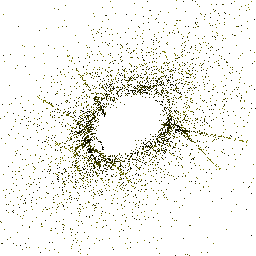
\includegraphics[width=\textwidth]{img/nbody.png}
    \caption{$N$-body}
    \label{fig:nbody}
  \end{subfigure}
  \begin{subfigure}{0.24\textwidth}
    
\includegraphics[width=\textwidth]{img/fluid.png}
    \caption{Fluid}
    \label{fig:fluid}
  \end{subfigure}
  \begin{subfigure}{0.24\textwidth}
    
\includegraphics[width=\textwidth]{img/crystal.png}
    \caption{Crystal}
    \label{fig:crystal}
  \end{subfigure}

  \caption{Visualisations of four benchmark programs implemented in
    Futhark, and called from Python.}
  \label{fig:visualisations}
\end{figure}


\section{Related Work on Automatic Parallelisation}

This section discusses three simplified Fortran 77 examples from the
DYFESM and BDNA benchmarks of the PERFECT club
suite~\cite{Berry88theperfect}, whose automatic parallelisation
requires complex compiler
analysis~\cite{CosPLDI,CIVan,OanceaMon}---for example based on (i)
inter-procedural summarization of array references, (ii) extraction of
runtime (sufficient) conditions for safe parallelization, and (iii)
special treatment of a class of induction variables (CIV) that cannot
be expressed as a closed-form formula in terms of loop indices.
%
Such analysis are beyond the capability of the common programmers and
commercial compilers, and it would not be necessary if application
parallelism was expressed explicitly by means of bulk-parallel
operators, as in a data-parallel language.

The first example, presented in Section~\ref{subsec:eg1}, semantically
corresponds to a map applied to an irregular two-dimensional array,
but the low level implementation---which uses indirect arrays,
unspecified preconditions, and array reshaping at call
sites----complicates analysis.

The second example, presented in Section~\ref{subsec:eg2}, shows an
example in which the same loop may encode two semantically different
parallel operators: a map and a generalized reduction.  Further
difficulties refer to the compiler having to reverse engineer users
optimizations, such as mapping two semantically different arrays to
the same memory block.

The third example, presented in Section~\ref{subsec:eg3}, shows a loop
that semantically corresponds to the sequential composition of a
filter and a map.  In this case the analysis has to be extended to (i)
accommodate ``conditional-induction variables'' (CIV), and to (ii)
reverse-engineer a composition of parallel-operators that is
semantically equivalent with the original sequential loop.

\subsection{Example 1: Difficult to Parallelise Map}
\label{subsec:eg1}

\begin{figure}[bt]

\begin{lstlisting}[language=fortran]
SUBROUTINE solvh(HE,XE,IA,IB)     SUBROUTINE geteu(XE,SYM,NP)
 DIMENSION  HE(32, *), XE(*)       DIMENSION  XE(16,*)
 READ(*,*) SYM, NS, NP, N
 CCC    SOLVH_do20
 DO i = 1, N, 1                     DO i = 1, NP, 1
  DO k = 1, IA(i), 1                 DO j = 1, 16, 1
   id = IB(i) + k - 1                 XE(j, i) = ...
   CALL geteu    (XE, SYM,  NP)      ENDDO
   CALL matmult(HE(1,id),XE,NS)     ENDDO
   CALL solvhe   (HE(1,id), NP)
  ENDDO                           END
ENDDO END
                                  SUBROUTINE solvhe(HE,NP)
SUBROUTINE matmult(HE,XE,NS)       DIMENSION  HE(8, *)
  DIMENSION HE(*), XE(*)
                                   DO j = 1, 3, 1
  DO j = 1, NS, 1                   DO i = 1, NP, 1
    HE(j) = XE(j)                    HE(j, i)=HE(j, i)+..
    XE(j) = ...                     ENDDO
ENDDO END                         ENDDO END
\end{lstlisting}

\caption{Simplified Loop SOLVH\_DO20 from DYFESM.}
\label{fig:SolvhDO20Code}
\end{figure}

\Cref{fig:SolvhDO20Code} shows the simplified version of loop
\texttt{solvh\_do20} from DYFESM benchmark of the PERFECT club
benchmark suite.
%
The aim is to prove that the (outermost) loop \texttt{solvh\_do20} is
parallel, in the sense that no dependencies exists between loop
iterations---in essence the loop is semantically an irregular
\texttt{map}, each iteration of it producing non-overlapping subsets
of the elements of the \texttt{XE} and \texttt{HE} arrays.

The reasoning necessary for proving loop \texttt{solvh\_do20} parallel
is nontrivial~\cite{CosPLDI}, and in fact impossible using purely
static techniques.  The presence of exploitable parallelism is
dependent on the statically unknown accesses using the indirect arrays
\texttt{IA} and \texttt{IB}, which semantically model irregular 2D
arrays.

The reasoning can proceed by looking at \texttt{XE} and \texttt{HE} as
unidimensional arrays, and by observing that \texttt{XE} is written in
subroutine \texttt{geteu} on all indexes belonging to interval
\texttt{[1,16*NP]} and is read in \texttt{matmult} on indexes in
\texttt{[1,NS]}.

Similarly, \texttt{HE} is written in \texttt{matmult} on all indexes in interval
\texttt{[$\tau$+1,$\tau$+NS]}, and read and written in \texttt{solvhe} on a subset
of indexes in interval \texttt{[$\tau$+1,$\tau$+8*NP-5]}, where
$\tau$\texttt{=32*(id-1)} is the array offset of parameter \texttt{HE(1,id)}.

\textit{Read-After-Write independence} of the outermost loop can be
established by showing that the per-iteration read set of \texttt{XE}
and \texttt{HE} are covered by their per-iteration write set. This
corresponds to solving interval-inclusion equations
\[
  \texttt{[1,NS]$\subseteq$[1,16*NP]}
\]
and
\[
  \texttt{[$\tau$+1,$\tau$+8*NP-5]$\subseteq$[$\tau$+1,$\tau$+NS]},
\]
yielding predicate
\[
  \texttt{NS$\leq$16*NP $\wedge$ 8*NP$<$NS+6}
\]
as sufficient condition for the flow independence of arrays
\texttt{XE} and \texttt{HE}, respectively.

For \textit{Write-After-Write independence}, one can observe that the
per-iteration write set of array \texttt{XE} is invariant to the
outermost loop, hence \texttt{XE} can be privatised and updated at the
very end with the values written by the last iteration (i.e.,
static-last value).

The rationale for the write-after-write independence of array
\texttt{HE} is more complicated: The write set of an iteration
\texttt{i} of loop \texttt{solvh\_do20},
denoted \texttt{WF$_i$}, can be overestimated to the interval of indices:
\[
  \texttt{[32*(IB(i)-1),32*(IB(i)+IA(i)-2)+NS-1]}
  \]
  The aim is to show that
  \[
    \forall i \neq j, \ \mbox{\texttt{WF}}_i \ \cap
    \mbox{\texttt{WF}}_j \ = \ \emptyset
\]
A sufficient condition~\cite{OanceaMon} that works in practice is
derived by checking the monotonicity of such intervals, i.e., the
upper bound of \texttt{WF$_i$} is less than than lower bound of
\texttt{WF$_{i+1}$}, for all $i$.
This results in the predicate
\[
  \wedge_{i=1}^{N-1}\texttt{NS$\leq$32*(IB(i+1)-IA(i)-IB(i)+1)}
\]
that verifies output independence under $O(\texttt{N})$ runtime
complexity.

\subsection{Example 2: Reduction or Map?}
\label{subsec:eg2}

Imperative techniques typically identify generalized-reduction
patterns on an array (or scalar) variable \texttt{A} by checking that
all its uses inside the target loop are of the form \texttt{A[x] =
  A[x] $\oplus$..}, where \texttt{x} is an arbitrary expression and
$\oplus$ is a (known) binary associative operator.

The code below is an example of a generalized reduction, and can be
parallelized by by computing the changes to \texttt{A} locally on each
processor and by merging (adding) them in parallel at the end of the
loop.

\begin{lstlisting}[language=fortran]
DO i = 1, N, 1
    A(B(i)) = A(B(i)) + C(i)
ENDDO
\end{lstlisting}

However, if \texttt{B} is an injective mapping of indices, this
treatment is unnecessary because each iteration reads and writes
distinct elements of \texttt{A}, and thus each processor can work
safely directly on the shared array \texttt{A}.  In Futhark terms, in
the latter case the loop is actually a composition of the parallel
operators \kw{map} and \kw{scatter}.

Identifying the case when a generalized reduction is a map can
requires summarization of the iteration-wise read-write set of the
target array \texttt{A}, denoted \texttt{RW$_i$} and checking that
they do not overlap.  This can be stated as the following equality:
\[
  \cup_{i=1}^{N}(\texttt{RW}_i\cap\cup_{k=1}^{i-1}(\texttt{RW}_k))=\emptyset
\]
Finally, sufficient conditions for identifying the \kw{map} case can
be extracted from this equation, for example by sorting the
\texttt{RW$_i$} sets (as intervals), and then checking
non-overlap. Such analysis is known as \textit{runtime reduction}
(RRED) in the literature~\cite{CosPLDI}, but it would not be necessary
if the map-scatter parallelism would be explicitly expressed in the
first place.

Another significant challenge to automatic parallelization are
memory optimizations performed by the programmer. The classical
example is privatization -- an analysis that determines whether
it is safe that the declaration of a variable is moved from outside
to inside the loop.   Another example is when two semantically
different arrays are combined into the same array, as 
illustrated in the example below. 

\begin{lstlisting}[language=fortran]
      DO i = 1, N, 1
S1:       A(i) = C(i)*2
S2:       A(B(i)) = A(B(i)) + C(i)
\end{lstlisting}

The statements \texttt{S1} and \texttt{S2} semantically build two different
arrays: one which is constructed by a map operation, and another
by a generalized-reduction operation.

To disambiguate such cases, compiler analysis needs to support an
extended reduction pattern (EXT-RRED), where the target array
\texttt{A} is allowed to be (only) written outside reduction
statements, as long as the write accesses do not precede on any
control-flow-graph path any reduction statement.  Note that instances
of EXT-RRED have non-empty per-iteration write-first (\texttt{WF$_i$})
and read-write (\texttt{RW$_i$}) sets and empty read-only set.

Enabling parallel execution in this case requires proving:
\begin{itemize}
\item Read-After-Write independence: \texttt{$\cup_{i=1}^N$(WF$_i$)
    $\cap$ $\cup_{i=1}^{N}$(RW$_i$)=$\emptyset$}, and either
\item Write-After-Write independence:
  $\cup_{i=1}^{N}(\texttt{WF}_i \cap \cup_{k=1}^{i-1}(\texttt{WF}_k))=\emptyset$ or
\item privatisation by static-last value:
  $\cup_{i=1}^{N}(\texttt{WF}_i) \subseteq\texttt{WF}_{i\leftarrow N}$
\end{itemize}

Loops MXMULT\_DO10 and FORMR\_DO20 that cover almost $55\%$ of
DYFESM's sequential runtime, exhibit both patterns discussed in this
section.

\subsection{Example 3: Conditional Induction Variables}
\label{subsec:eg3}

Another challenge for automatic parallelisation are the so called
``conditional-induction variables'' (CIV) that represent scalars that
do not form a uniform recurrence, e.g., their increment is not
constant across the iteration space of the analysed loop.

\begin{lstlisting}[language=fortran,mathescape=true,escapechar=|]
    civ@1 = 0
    DO i = 1, N, 1
      civ@2=$\phi$(civ@1, civ@4)
      IF C(i) .GT. 0 THEN
        DO j = 1, C(i), 1
          X(j+civ@2) = ...
        ENDDO
        civ@3 = C(i) + civ@2
      ENDIF
      civ@4 = $\phi$(civ@3, civ@2)
    ENDDO
    civ@5=$\phi$(civ@4, civ@1)
\end{lstlisting}

The code above shows a simplified version of loop
\texttt{CORREC\_do401} from BDNA benchmark, as an example of
non-trivial loop that uses both CIV and affine-based subscripts.
Variable \texttt{civ} is written directly in (gated)
single-static-assignment (SSA) notation.

For example, statement \texttt{civ@2=$\phi$(civ@1,civ@4)} has the
semantics that variable \texttt{civ@2} takes either the value of
\texttt{civ@1} for the first iteration of the loop or the value of
\texttt{civ@4} for all other iterations.

The gist of the parallelisation technique~\cite{CIVan} is to aggregate
symbolically the CIV references on every control-flow path of the
analyzed loop, in terms of the CIV values at the entry and end of each
iteration or loop.  The analysis succeeds if (i) the symbolic-summary
results are identical on all paths and (ii) they can be aggregated
across iterations in the interval domain.
%
Parallelisation requires two main steps:
\begin{itemize}
    \item[1] proving the absence of cross-iteration dependencies 
        on array \texttt{X}. 
%        do not raise any cross-iteration dependencies,
%        by symbolically expressing read/write (index) 
%        summaries in terms of \texttt{civ@2} and \texttt{civ@4} 
%        and by using the monotonicity of \texttt{civ@2}
%        values across across iterations, and
    \item[2] computing in parallel the values of \texttt{civ}
    at the beginning of each iteration, i.e., the values of \texttt{civ@2}. 
\end{itemize}

\paragraph{Step 1.} 
The write accesses of the inner loop can be summarized
by the interval
\[
  \texttt{WF$_{inner-loop}$=[civ@2,civ@2+C(i)-1]}.
\]
On the path on which condition \texttt{C(i).GT.0} holds, we have
\[
  \texttt{civ@4$=$civ@3$=$civ@2+C(i)}
\]
and the path summary is
rewritten as
\[
  \texttt{W$_i^{THEN}$ = [civ@2,civ@4-1]}.
\]

The other path neither updates \texttt{X} nor increments \texttt{civ},
hence it can use the same symbolic summary
\[
  \texttt{W}_i^{ELSE} = \texttt{[civ@2,civ@4-1]} = \emptyset
  \]
because on that path \texttt{civ@2=civ@4>civ@4-1}, and an interval
having its lower bound greater than its upper bound is considered
empty.

It follows that the summaries of the \texttt{THEN} and \texttt{ELSE} branches
can be unified; the iteration summary being
\[
  \texttt{$W_i$~=~[civ@2,civ@4-1]}.
\]

Loop independence can now be proven by verifying the set equation
\[
  \texttt{$\cup_{i=1}^{N}$(W$_i$ $\cap$ $\cup_{k=1}^{i-1}$(WF$_k$))=$\emptyset$},
\]
which holds because \texttt{$\cup_{k=1}^{i-1}$(WF$_k$)} can be symbolically
computed to be \texttt{[1, civ@2$^i$-1]} by using:
\begin{itemize}
\item the implicit invariant
  $\texttt{civ@4}^{i-1}=\texttt{civ@2}^{i}$, i.e., the \texttt{civ}
  value at an iteration end is equal to the \texttt{civ} value at the
  entry of the next iteration, and
\item the monotonicity of the \texttt{civ@2} values (because they are
  incremented by \texttt{C(i)} only when \texttt{C(i)} is positive).
\end{itemize}

\paragraph{Step 2.} While the accesses to \texttt{X} have been
disambiguated, \texttt{civ} still remains the source of cross
iteration dependences.

The CIV values at the beginning of each iteration can be computed in
parallel by the following technique:
%
First, the slice that computes \texttt{civ} in an iteration is
extracted and it is checked that \texttt{civ} appears only in
reductions statement in it. Second, the \texttt{civ@2} is initialized
(in the slice) to the neutral-element of the reduction
operator. Third, the obtained slice is mapped across the original
iterations space, and the result is subjected to an exclusive scan.

The Futhark code below illustrates the result of this technique on our
example\footnote{Except that \kw{scan} in Futhark is inclusive, not
  exclusive.}:

\begin{lstlisting}
scan (+) 0 (map (\i -> if C[i] > 0 then C[i] else 0)
                [1...N])
\end{lstlisting}

We conclude by remarking that in addition to this ``heroic'' analysis,
which is necessary for proving the absence of cross-iteration
dependences for array \texttt{X} that uses CIV-based accesses, the
compiler also had to re-engineer the computation of \texttt{civ}
values from inherently sequential to parallel.  We argue that, if
parallel execution is desired, the code should have been written from
the very beginning in terms of data-parallel operators rather than
sequential loops.

\section{Related Work on Data-Parallel Languages}

Fortunately, not all work on parallelism involves Fortran 77.  There
is a rich body of literature on embedded array languages and libraries
targetting GPUs. Imperative solutions include
Copperhead~\cite{Copperhead}, Accelerator~\cite{MSaccelerator}, and
deep-learning DSLs, such as Theano~\cite{Theano} and
Torch~\cite{Torch7}.

Purely functional languages include
Accelerate~\cite{mcdonell2013optimising},
Obsidian~\cite{claessen2012expressive}, and
NOVA~\cite{collins2014nova}.  These languages support neither
arbitrary nested regular parallelism, nor explicit indexing and
efficient sequential code inside their parallel constructs.

A number of dataflow languages aim at efficient GPU compilation.
StreamIt supports a number of static optimizations on various
hardware, for example, GPU
optimizations~\cite{Hormati:2011:SPS:1950365.1950409} include
memory-layout selection (shared/global memory), resolving
shared-memory bank conflicts, increasing the granularity of
parallelism by vertical fusion, and untilizing unused registers by
software prefetching and loop unrolling, while multicore
optimizations~\cite{Gordon:2006:ECT:1168857.1168877} are aimed at
finding the right mix of task, data and pipeline parallelism.

Finally, we note that Futhark is not intended as a general-purpose
language, but rather it is aimed at (i) expressing computational
kernels, which can then be linked with applications written in
mainstream languages, and, at (ii) being used as a code-generation
target for high-level DSLs.  Such a usage was demonstrated by an
experiment~\cite{ElsmanDybdal:Array:2014,Henriksen:2016:AGT:2975991.2975997}
in which a subset of APL was compiled to Futhark, executed on GPU, and
used from Python for visualization purposes.


%%% Local Variables:
%%% mode: latex
%%% TeX-master: "thesis"
%%% End:
